\documentclass[12pt]{letter}\usepackage[letterpaper,margin=0.65in]{geometry}\usepackage{textcomp}\usepackage{graphicx}\usepackage[rflt]{floatflt}\pagenumbering{gobble}\begin{document}\begin{floatingfigure}{0.15\textwidth}\raisebox{0pt}[0pt][0pt]{\raisebox{-2.5cm}{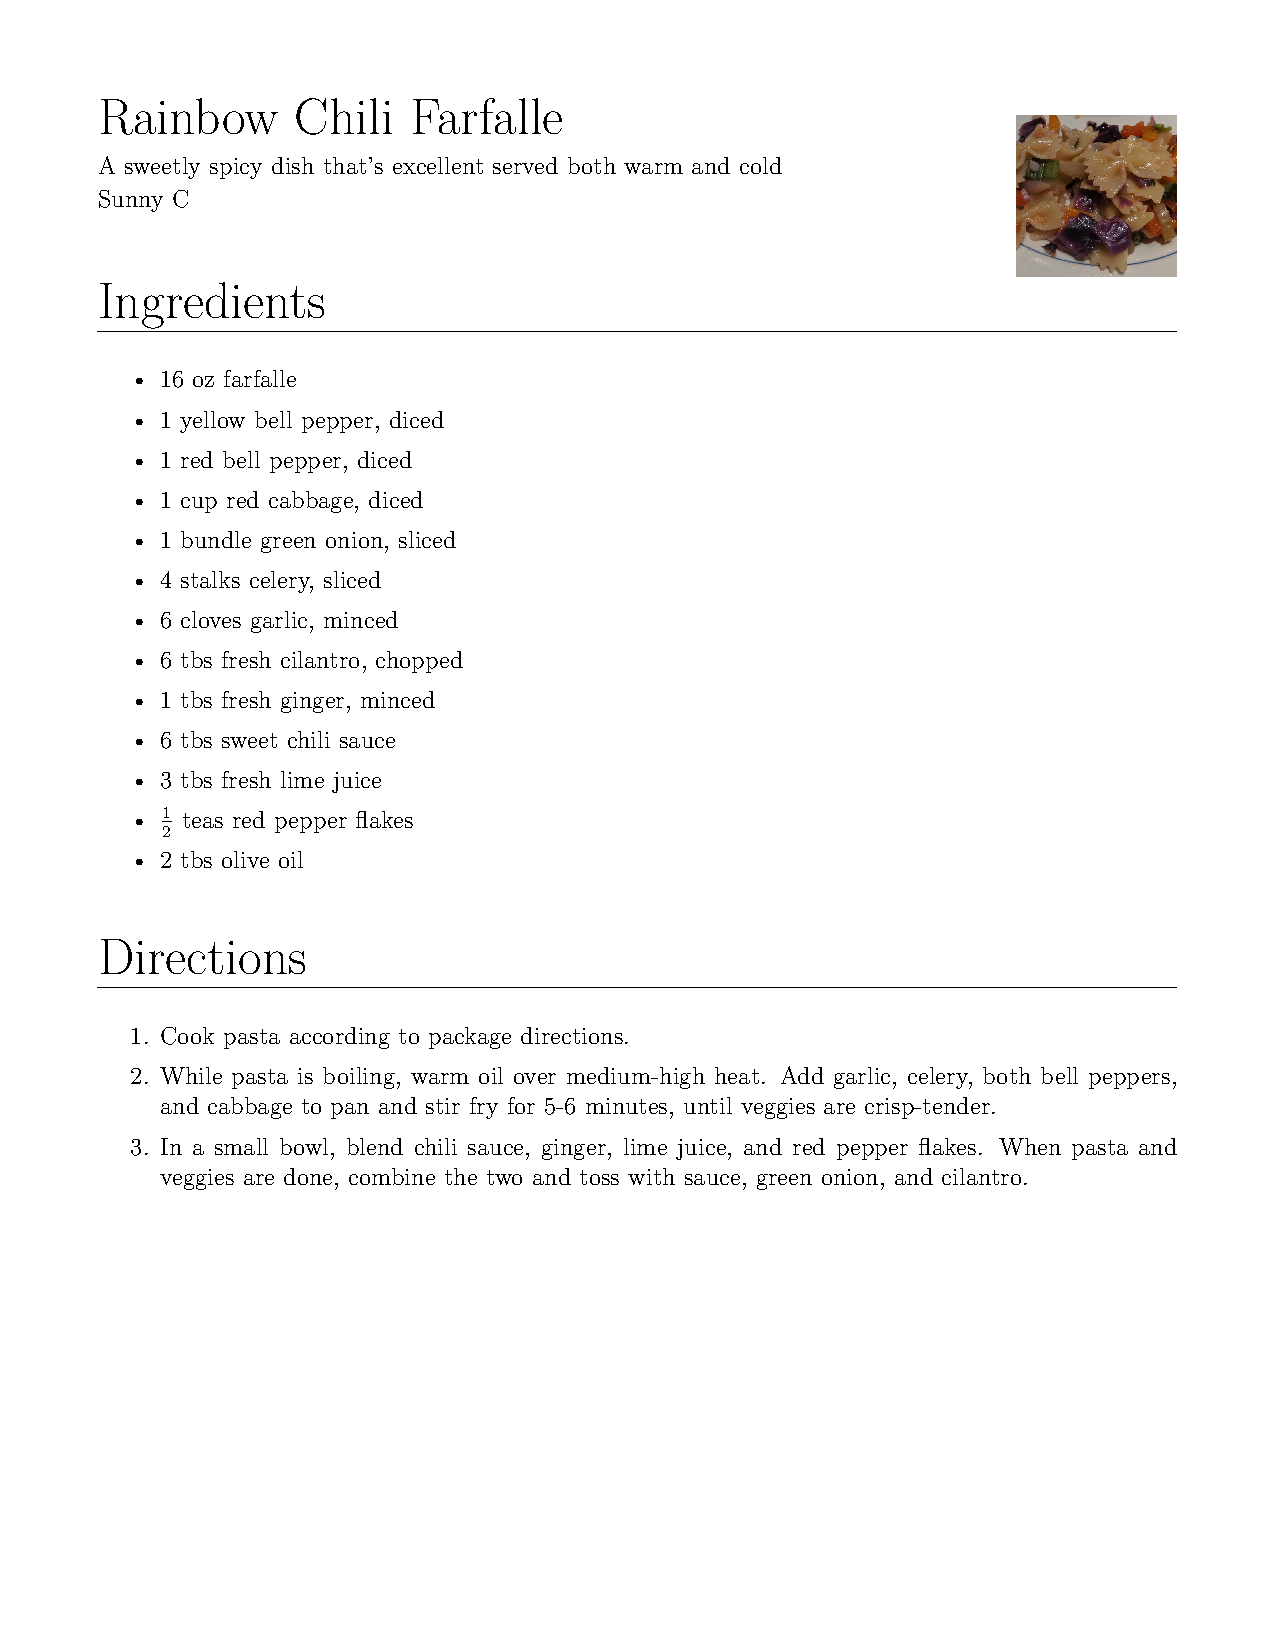
\includegraphics[width=0.15\textwidth]{rainbow-chili-farfalle}}}\end{floatingfigure}\begin{huge}Rainbow Chili Farfalle\end{huge}\newline\vspace{-2.5mm}\newline\renewcommand{\arraystretch}{1.1}\begin{tabular*}{\textwidth}{@{\extracolsep{\fill}}lr}A sweetly spicy dish that's excellent served both warm and cold\\Sunny C\end{tabular*}\newline\vspace{10mm}\newline\begin{huge}Ingredients\end{huge}\\\rule[2.8mm]{\textwidth}{.1pt}\vspace{-3mm}\begin{itemize}\item 16 oz farfalle\item 1 yellow bell pepper, diced\item 1 red bell pepper, diced\item 1 cup red cabbage, diced\item 1 bundle green onion, sliced\item 4 stalks celery, sliced\item 6 cloves garlic, minced\item 6 tbs fresh cilantro, chopped\item 1 tbs fresh ginger, minced\item 6 tbs sweet chili sauce\item 3 tbs fresh lime juice\item $\frac{1}{2}$ teas red pepper flakes\item 2 tbs olive oil\end{itemize}\vspace{7mm}\begin{huge}Directions\end{huge}\\\rule[2.8mm]{\textwidth}{.1pt}\vspace{-3mm}\begin{enumerate}\item Cook pasta according to package directions.\item While pasta is boiling, warm oil over medium-high heat. Add garlic, celery, both bell peppers, and cabbage to pan and stir fry for 5-6 minutes, until veggies are crisp-tender.\item In a small bowl, blend chili sauce, ginger, lime juice, and red pepper flakes. When pasta and veggies are done, combine the two and toss with sauce, green onion, and cilantro.\end{enumerate}\end{document}